% Main LaTeX Document for DeepMTL2R Paper
% Reorganized with modular structure
% 
% This is the main entry point. Compile this file with:
%   pdflatex main.tex && bibtex main.tex && pdflatex main.tex && pdflatex main.tex
\documentclass[11pt]{article}
% Load configuration and packages from preamble
\input{preamble.tex}
% ============================================================================
% Document Metadata
% ============================================================================
\title{Extending DeepMTL2R: Multi-Task Learning to Rank with Dynamic Feature Gating and Matryoshka Feature Projection}
% Author information
\author{Jeslyn Theodora \\
  Faculty of Computer Science \\
  University of Indonesia \\
  \texttt{jeslyn.theodora@ui.ac.id} \\\And
  Maulana Seto \\
  Faculty of Computer Science \\
  University of Indonesia \\
  \texttt{maulana.seto@ui.ac.id} \\}
% ============================================================================
% Document Content
% ============================================================================
\begin{document}

% Abstract
\begin{abstract}
Multi-task Learning to Rank (MTL2R) jointly optimizes multiple ranking criteria, allowing models to capture diverse aspects of document quality beyond a single relevance signal. This paper extends the DeepMTL2R framework through two architectural modifications, namely \textbf{Dynamic Feature Gating} (DFG), which employs a sigmoid-activated learnable mask over input features to suppress low-information dimensions, and \textbf{Matryoshka Feature Projection} (MFP), which reorganizes the output layer to generate nested representations that can be sliced at inference time without retraining. Both extensions are evaluated on the MSLR-WEB10K benchmark under six task-weight configurations across two folds. Experiments reveal a critical numerical failure in which the listwise LambdaLoss gain function $2^{y}-1$ exceeds \texttt{float32} precision when applied to unnormalized auxiliary targets, producing \texttt{NaN} gradients from the first epoch and freezing all model weights at their initialized values. Consequently, both DFG and MFP are unable to demonstrate their intended benefits. We identify target normalization and task-specific loss decoupling as the primary remedies, and discuss their implications for future work.
\end{abstract}

\maketitle
% ============================================================================
% Main Content Sections
% ============================================================================
% Section: Introduction
\section{Introduction}

Learning to Rank (LTR) is a foundational component of modern information retrieval systems, underpinning applications such as web search engines and recommendation systems. Traditionally, LTR techniques optimize for a single objective, such as relevance \cite{yan2023learningrankgradesmatter}. However, real-world ranking environments must balance multiple noisy, subjective, and heterogeneous signals. Multi-Task Learning to Rank (MTL2R) addresses this challenge by jointly modeling auxiliary criteria \cite{Caruana1997MultitaskL}, allowing ranking decisions to better reflect diverse facets of document quality and search intent.

DeepMTL2R is an open-source deep learning library that implements MTL2R via self-attention mechanisms in transformer architectures \cite{dong2026deepmtl2rlibrarydeepmultitask}. However, its core architecture has two limitations: it lacks explicit feature selection (recent CTR architectures show gating masks improve representation quality and interpretability \cite{huang2020gatenet,wang2021masknet}), and its fixed-dimension output cannot serve rankings at different granularities. In commercial multi-stage retrieval pipelines \cite{covington2016deep}, this forces practitioners to either maintain multiple separate models or compromise on retrieval latency.

To address these limitations, we introduce two architectural extensions to the DeepMTL2R framework:\footnote{Our implementation is available at: \href{https://github.com/jteo0/DeepMTL2R}{\texttt{github.com/jteo0/DeepMTL2R}}}
\begin{itemize}
    \item \textbf{Dynamic Feature Gating} introduces a sigmoid-activated linear mask prior to the input projection layer to suppress low-information features dynamically during training, inspired by gating networks \cite{huang2020gatenet,wang2021masknet}.
    \item \textbf{Matryoshka Feature Projection} restructures the output layer to enforce Matryoshka Representation Learning (MRL) \cite{kusupati2022matryoshka}, allowing the model to produce nested embeddings that can be adaptively sliced at inference without retraining.
\end{itemize}

Both extensions are evaluated against the DeepMTL2R baseline on the MSLR-WEB10K dataset under six task-weight configurations, reporting NDCG at multiple cutoffs, MAP@10, and MRR@10. We further analyze gating sparsity, noise robustness, and the dimensional efficiency of Matryoshka representations across nesting dimensions $\mathcal{M} = \{32, 64, 128, 256\}$.
\section{Method}

\subsection{System Architecture}

Both extensions are built on the DeepMTL2R framework, whose baseline pipeline consists of an input layer, a transformer encoder, and a task-specific output layer, as illustrated in Figure~\ref{fig:baselinepipeline}. Input features are first projected through a shared \texttt{FCModel}, then encoded using self-attention \cite{vaswani2017attention} across the query slate, and finally passed to task-specific linear heads that each generate a scalar relevance score.
\begin{figure}[!htbp]
  \centering
  \includegraphics[width=\columnwidth]{images/DeepMTL2R.png}
  \caption{DeepMTL2R baseline pipeline.}
  \label{fig:baselinepipeline}
\end{figure}

\subsubsection{Dynamic Feature Gating}

Dynamic Feature Gating introduces a trainable gating mechanism directly before \texttt{FCModel}, acting as a soft feature-selection mask, as shown in Figure~\ref{fig:featuregating}.
\begin{figure}[!htbp]
  \centering
  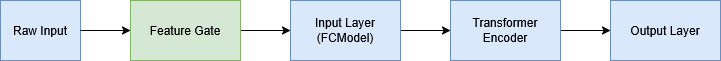
\includegraphics[width=\columnwidth]{images/FeatureGating.png}
  \caption{DeepMTL2R architecture modified with Dynamic
  Feature Gating.}
  \label{fig:featuregating}
\end{figure}

Let $\mathbf{x} \in \mathbb{R}^d$ denote the raw input feature vector with dimensionality $d = 133$. A linear transformation followed by a sigmoid activation is applied to generate the gating mask, given by
\begin{equation}
  \mathbf{g} = \sigma(\mathbf{W}_g \mathbf{x} +
  \mathbf{b}_g), \quad \mathbf{g} \in [0, 1]^d\text{,}
\end{equation}
after which the gated representation is obtained through the element-wise Hadamard product
\begin{equation}
  \mathbf{\tilde{x}} = \mathbf{g} \odot \mathbf{x}\text{.}
\end{equation}

\subsubsection{Matryoshka Feature Projection}

Matryoshka Feature Projection integrates Matryoshka
Representation Learning (MRL) \cite{kusupati2022matryoshka}
into the output projection layer
(Figure~\ref{fig:matryoshka}), widening the encoder
hidden size to $D = 256$ and enforcing coarse-to-fine
encoding via nested prefix slices.

\begin{figure}[!htbp]
  \centering
  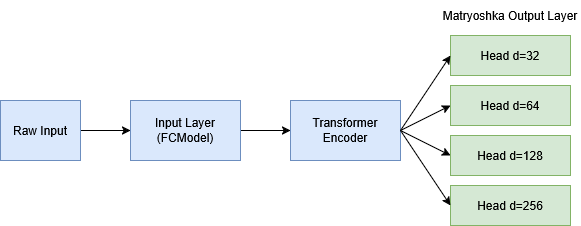
\includegraphics[width=\columnwidth]{images/Matryoshka.png}
  \caption{DeepMTL2R architecture modified with
  Matryoshka Feature Projection.}
  \label{fig:matryoshka}
\end{figure}

For nesting dimensions $\mathcal{M} = \{32, 64, 128, 256\}$, each slice $\mathbf{h}^{(m)} = \mathbf{h}_{1:m}$ is connected to a task-specific linear prediction head such that
\begin{equation}
  \hat{y}_t^{(m)} = \mathbf{w}_{t}^{(m)\top}
  \mathbf{h}^{(m)} + b_t^{(m)} \text{,}
\end{equation}
where $t \in \mathcal{T} = \{0,1,2,3\}$. The overall training objective is then obtained by aggregating the losses across all nesting dimensions and tasks, yielding
\begin{equation}
  \mathcal{L}_{\text{total}} = \sum_{m \in \mathcal{M}}
  \sum_{t \in \mathcal{T}} w_t \mathcal{L}_t\!\left(
  \hat{\mathbf{y}}_t^{(m)}, \mathbf{y}_t\right)\text{.}
\end{equation}
At inference time, only the full $D = 256$ slice is used by default, although lower-dimensional sub-vectors can still be extracted for latency-critical retrieval scenarios.

\subsection{Training Hyperparameters}

All architectures share the hyperparameters listed in
Table~\ref{tab:hyperparams}. Training uses the LambdaLoss framework \cite{wang2018lambdaloss} with \texttt{ndcgLoss2PP\_scheme} ($\mu=10$, $\sigma=1.0$), the Adam optimizer (lr $= 0.001$), and a batch size of 32 query slates over 50 epochs.

\begin{table}[h]
  \centering
  \caption{\label{tab:hyperparams}
    Training hyperparameters shared across all
    architectures.
  }
  \resizebox{\columnwidth}{!}{%
  \begin{tabular}{lll}
    \toprule
    \textbf{Hyperparameter} & \textbf{Value} &
    \textbf{Description} \\
    \midrule
    Epochs        & 50       & Max training epochs \\
    Batch size    & 32       & Query slates per batch \\
    Optimizer     & Adam     & Adapts learning rates
                               per parameter \\
    Learning rate & 0.001    & Initial LR \\
    LR scheduler  & StepLR  & \texttt{step\_size=50},
                               \texttt{gamma=0.1} \\
    Loss function & LambdaLoss &
                    \texttt{ndcgLoss2PP\_scheme},
                    $\mu=10$ \\
    \bottomrule
  \end{tabular}%
  }
\end{table}
% Section: Experiments
\section{Experiments}

\subsection{Experimental Dataset}

We evaluate our proposed methods on the MSLR-WEB10K dataset \cite{QinL13}, a standard and publicly available benchmark for learning-to-rank. The dataset consists of query-document slates, where each document has been labeled with a discrete relevance score ranging from 0 (irrelevant) to 4 (perfectly relevant) based on search engine queries.

Following a multi-task ranking setup, the 136 original features of MSLR-WEB10K are partitioned into input features and auxiliary targets, with three continuous features reserved as auxiliary target outputs
\begin{itemize}
    \item \textbf{Task 131 (QualityScore)}, corresponding to Feature 132 in the dataset, represents a document quality metric;
    \item \textbf{Task 132 (QualityScore2)}, corresponding to Feature 133 in the dataset, represents a secondary document quality metric; and
    \item \textbf{Task 133 (Query-URL click count)}, corresponding to Feature 134 in the dataset, represents historical user interaction frequency.
\end{itemize}
These three features are excluded from the model's feature space, leaving $d = 133$ features as model inputs. We evaluate all models across Fold 1 and Fold 2 of the dataset. For each fold, we train on the training split for exactly 50 epochs, monitor the validation set performance, and report the final metrics on the test split using the model state from the final training epoch.

\subsection{Models and Baselines}
To assess the effectiveness of Dynamic Feature Gating (DFG) and Matryoshka Feature Projection (MFP), we compare four models consisting of two baselines and two proposed extensions.

\begin{enumerate}
    \item \textbf{Single-Task Baseline} represents the
    standard DeepMTL2R pipeline trained exclusively on
    the primary relevance objective (Task~0), without
    incorporating auxiliary supervision.

    \item \textbf{Vanilla Multi-Task Baseline}
    corresponds to the original DeepMTL2R framework
    jointly optimized across all four tasks using equal
    loss weighting ($[1.0, 1.0, 1.0, 1.0]$).

    \item \textbf{Dynamic Feature Gating (DFG)}
    extends DeepMTL2R with a learnable soft gating mask
    applied to the 133 input features before the feature
    projection stage.

    \item \textbf{Matryoshka Feature Projection (MFP)}
    modifies the framework by introducing nested
    representation slicing at the output layer across
    dimensions $\mathcal{M} = \{32, 64, 128, 256\}$.
\end{enumerate}

\subsection{Multi-Task Weight Configurations}

To map the Pareto frontier of multi-task performance, both extension models (DFG and MFP) are trained across six distinct task-weight configurations $\mathbf{w} = [w_0, w_1, w_2, w_3]$ as detailed in Table~\ref{tab:weights}, where $w_0$ represents the weight of the primary task and $w_1, w_2, w_3$ represent the weights of the auxiliary tasks. These weights are scalarized linearly as training objectives, meaning the overall loss function is computed as the weighted sum of the individual task losses ($L_{total} = \sum_{i=0}^{3} w_i L_i$).

Consequently, assigning a higher weight to a specific task forces the model to prioritize minimizing its loss, effectively steering the learning capacity toward that signal. The vanilla multi-task baseline is trained using uniform task weights scaled to $[1.0, 1.0, 1.0, 1.0]$, representing an equivalent ratio to $W_0$.

\begin{table}[!htbp]
  \centering
  \caption{\label{tab:weights} Task weight configurations for linear scalarization.}
  \resizebox{\columnwidth}{!}{%
  \begin{tabular}{ccl}
    \toprule
    \textbf{Configuration} & \textbf{Weights} $[w_0, w_1, w_2, w_3]$ & \textbf{Description} \\
    \midrule
    $W_0$ & $[0.25, 0.25, 0.25, 0.25]$ & Uniform task weighting \\
    $W_1$ & $[0.70, 0.10, 0.10, 0.10]$ & Main task highly focused \\
    $W_2$ & $[0.40, 0.20, 0.20, 0.20]$ & Main task moderately focused \\
    $W_3$ & $[0.10, 0.70, 0.10, 0.10]$ & QualityScore (Task 1) focused \\
    $W_4$ & $[0.10, 0.10, 0.70, 0.10]$ & QualityScore2 (Task 2) focused \\
    $W_5$ & $[0.10, 0.10, 0.10, 0.70]$ & Click count (Task 3) focused \\
    \bottomrule
  \end{tabular}%
  }
\end{table}

\subsection{Evaluation Metrics}

We evaluate the ranking performance of the models using several standard LTR and multi-task metrics.

\begin{itemize}
    \item \textbf{NDCG@k} denotes the Normalized Discounted Cumulative Gain evaluated at cutoff ranks $k \in \{1, 5, 10, 20, 30\}$. Among these, NDCG@10 on the primary task (Task~0) is monitored on the validation split during training and used as the primary comparison metric.
    \item \textbf{MAP@10} represents the Mean Average Precision computed at rank 10 on the primary task.
    \item \textbf{MRR@10} corresponds to the Mean Reciprocal Rank evaluated at rank 10 on the primary task.
    \item \textbf{Noise Robustness Drop} measures the resilience of the models under noisy input conditions by injecting zero-mean Gaussian noise $\epsilon \sim \mathcal{N}(0, \sigma^2)$ into the feature vectors, where $\sigma^2$ is fixed at $10\%$ of the feature variance. Both absolute and relative percentage drops are computed across all evaluation metrics, including NDCG at all cutoffs, MAP, and MRR, to assess multi-task ranking robustness.
    \item \textbf{Dimensional Efficiency (MFP only)} evaluates partial slices of the Matryoshka output representations at dimensions 32, 64, and 128 to determine how effectively lower-dimensional embeddings preserve ranking performance.
\end{itemize}
% Section: Results and Evaluation
\section{Results and Evaluation}

\subsection{Quantitative Ranking Results}

The experimental results for the MSLR-WEB10K ranking tasks across all models are summarized in Table~\ref{tab:results_primary} for the primary task and Table~\ref{tab:results_auxiliary} for the auxiliary tasks. The primary task (Task~0) is evaluated using NDCG at multiple cutoff ranks, while the auxiliary tasks (Tasks~131, 132, 133) are evaluated using NDCG@10 and NDCG@30. Task~132 NDCG values for the Multi-Task Baseline are undefined (\texttt{NaN}) for Fold~2 due to a degenerate slate where all documents share identical relevance labels; only Fold~1 values are reported.

\begin{table}[!htbp]
  \centering
  \caption{\label{tab:results_primary} Primary task (Task~0) NDCG scores averaged over Folds 1
  and 2 on the test split.}
  \resizebox{\columnwidth}{!}{%
  \begin{tabular}{lccccc}
    \toprule
    \textbf{Model / Config} & \textbf{NDCG@1} & \textbf{NDCG@5} & \textbf{NDCG@10}
    & \textbf{NDCG@20} & \textbf{NDCG@30} \\
    \midrule
    Single-Task Baseline    & $0.0714$ & $0.6836$ & $0.6836$ & $0.6836$ & $0.6836$ \\
    Multi-Task Baseline     & $0.5000$ & $0.8155$ & $0.8155$ & $0.8155$ & $0.8155$ \\
    \midrule
    \multicolumn{6}{l}{\textbf{Dynamic Feature Gating (DFG)}} \\
    \quad $W_0$ & $0.1520$ & $0.1822$ & $0.2122$ & $0.2588$ & $0.2997$ \\
    \quad $W_1$ & $0.1520$ & $0.1822$ & $0.2122$ & $0.2588$ & $0.2998$ \\
    \quad $W_2$ & $0.1522$ & $0.1823$ & $0.2122$ & $0.2588$ & $0.2998$ \\
    \quad $W_3$ & $0.1520$ & $0.1822$ & $0.2122$ & $0.2588$ & $0.2998$ \\
    \quad $W_4$ & $0.1519$ & $0.1822$ & $0.2122$ & $0.2588$ & $0.2998$ \\
    \quad $W_5$ & $0.1519$ & $0.1821$ & $0.2122$ & $0.2588$ & $0.2998$ \\
    \midrule
    \multicolumn{6}{l}{\textbf{Matryoshka Feature Projection (MFP)}} \\
    \quad $W_0$ & $0.1520$ & $0.1822$ & $0.2122$ & $0.2588$ & $0.2998$ \\
    \quad $W_1$ & $0.1521$ & $0.1822$ & $0.2122$ & $0.2588$ & $0.2998$ \\
    \quad $W_2$ & $0.1521$ & $0.1822$ & $0.2122$ & $0.2588$ & $0.2998$ \\
    \quad $W_3$ & $0.1520$ & $0.1822$ & $0.2122$ & $0.2588$ & $0.2998$ \\
    \quad $W_4$ & $0.1520$ & $0.1822$ & $0.2122$ & $0.2588$ & $0.2998$ \\
    \quad $W_5$ & $0.1519$ & $0.1821$ & $0.2122$ & $0.2588$ & $0.2998$ \\
    \bottomrule
  \end{tabular}%
  }
\end{table}

\begin{table}[!htbp]
  \centering
  \caption{\label{tab:results_auxiliary} Auxiliary task NDCG scores averaged over Folds 1 and 2
  on the test split.}
  \resizebox{\columnwidth}{!}{%
  \begin{tabular}{lcccccc}
    \toprule
    \textbf{Model / Config} & \multicolumn{2}{c}{\textbf{Task 131}}
    & \multicolumn{2}{c}{\textbf{Task 132}} & \multicolumn{2}{c}{\textbf{Task 133}} \\
    \cmidrule(lr){2-3} \cmidrule(lr){4-5} \cmidrule(lr){6-7}
    & \textbf{@10} & \textbf{@30} & \textbf{@10} & \textbf{@30} & \textbf{@10} & \textbf{@30} \\
    \midrule
    Multi-Task Baseline & $0.5658$ & $0.5658$ & $0.5000^{\dagger}$
    & $0.5000^{\dagger}$ & $1.0000$ & $1.0000$ \\
    \midrule
    \multicolumn{7}{l}{\textbf{Dynamic Feature Gating (DFG)}} \\
    \quad $W_0$ & $0.2434$ & $0.3358$ & $0.2554$ & $0.3409$ & $0.3992$ & $0.4341$ \\
    \quad $W_1$ & $0.2434$ & $0.3358$ & $0.2554$ & $0.3409$ & $0.3992$ & $0.4341$ \\
    \quad $W_2$ & $0.2434$ & $0.3358$ & $0.2554$ & $0.3409$ & $0.3992$ & $0.4341$ \\
    \quad $W_3$ & $0.2434$ & $0.3357$ & $0.2554$ & $0.3409$ & $0.3992$ & $0.4341$ \\
    \quad $W_4$ & $0.2434$ & $0.3357$ & $0.2554$ & $0.3409$ & $0.3992$ & $0.4341$ \\
    \quad $W_5$ & $0.2434$ & $0.3357$ & $0.2554$ & $0.3409$ & $0.3992$ & $0.4341$ \\
    \midrule
    \multicolumn{7}{l}{\textbf{Matryoshka Feature Projection (MFP)}} \\
    \quad $W_0$ & $0.2434$ & $0.3358$ & $0.2554$ & $0.3461$ & $0.3992$ & $0.4341$ \\
    \quad $W_1$ & $0.2434$ & $0.3358$ & $0.2554$ & $0.3461$ & $0.3992$ & $0.4341$ \\
    \quad $W_2$ & $0.2434$ & $0.3358$ & $0.2554$ & $0.3461$ & $0.3992$ & $0.4341$ \\
    \quad $W_3$ & $0.2434$ & $0.3358$ & $0.2554$ & $0.3461$ & $0.3992$ & $0.4341$ \\
    \quad $W_4$ & $0.2434$ & $0.3357$ & $0.2554$ & $0.3461$ & $0.3992$ & $0.4341$ \\
    \quad $W_5$ & $0.2434$ & $0.3358$ & $0.2554$ & $0.3461$ & $0.3992$ & $0.4341$ \\
    \bottomrule
  \end{tabular}%
  }
  \par\smallskip
  {\footnotesize $^{\dagger}$Task~132 NDCG for the Multi-Task Baseline is reported from Fold~1 only; Fold~2 produced an undefined value due to a degenerate slate with uniform relevance labels.}
\end{table}

\begin{table}[!htbp]
  \centering
  \caption{\label{tab:baseline_folds} Per-fold NDCG@1 and NDCG@10 breakdown for baseline models on the primary task (Task~0).}
  \resizebox{\columnwidth}{!}{%
  \begin{tabular}{lcccccc}
    \toprule
    & \multicolumn{3}{c}{\textbf{NDCG@1}} & \multicolumn{3}{c}{\textbf{NDCG@10}} \\
    \cmidrule(lr){2-4} \cmidrule(lr){5-7}
    \textbf{Baseline Model} & \textbf{Fold 1} & \textbf{Fold 2} & \textbf{Average}
    & \textbf{Fold 1} & \textbf{Fold 2} & \textbf{Average} \\
    \midrule
    Single-Task Baseline & $0.0000$ & $0.1429$ & $0.0714$ & $0.6309$ & $0.7364$ & $0.6836$ \\
    Multi-Task Baseline  & $0.0000$ & $1.0000$ & $0.5000$ & $0.6309$ & $1.0000$ & $0.8155$ \\
    \bottomrule
  \end{tabular}%
  }
\end{table}

Table~\ref{tab:baseline_folds} presents the per-fold NDCG@1 and NDCG@10 results for the baseline models. The Single-Task Baseline achieved an average NDCG@10 of $0.6836$, whereas the Multi-Task Baseline reported a substantially higher average score of $0.8155$. Nevertheless, this apparent improvement is primarily caused by a dataset artifact. In Fold~2, the Multi-Task Baseline obtained a perfect score of $1.0000$ on the primary task, while Task~133 also reached exactly $1.0000$. This outcome arises from a tie-breaking artifact induced by the pre-sorted order of the Fold~2 test split rather than from meaningful ranking performance. By contrast, both baseline models produced identical results on Fold~1.

Both DFG and MFP models exhibited severely degraded ranking performance across all NDCG cutoffs, stagnant at NDCG@1~$\approx 0.152$, NDCG@10~$\approx 0.212$, and NDCG@30~$\approx 0.300$ across all weight configurations. Notably, scores are nearly identical across all six weight configurations ($W_0$--$W_5$) for both models; this uniformity is a direct consequence of the NaN gradient collapse described in Section~\ref{sec:nan}, which froze all model weights at their initialized values before any task-weight differences could take effect.

\subsection{Numerical Collapse Analysis (NaN Loss)}
\label{sec:nan}

All three models experienced a numerical collapse that produced \texttt{NaN} training losses from the first epoch and froze all weights at initialization. This failure originates from the \texttt{ndcgLoss2PP\_scheme} in the \texttt{allrank} library \cite{wang2018lambdaloss}, whose exponential gain function $2^{y}-1$ remains stable for primary task labels ($y \in [0,4]$) but overflows \texttt{float32} precision ($2^{128}$) when applied to unnormalized auxiliary targets such as click counts up to $13.15 \times 10^{6}$ and quality scores up to $254$, immediately producing \texttt{inf} and \texttt{NaN} gradients.

Because the DeepMTL2R framework enforces a uniform loss formulation across all tasks and lacks a built-in target normalization pipeline, applying it directly to standard datasets with continuous auxiliary targets inevitably triggers this overflow. Thus, this failure highlights a structural limitation in the baseline framework's multi-task loss handling, rather than an experimental oversight.

Despite the training collapse, validation metrics were still logged because we introduced a custom safeguard in \texttt{allrank/models/metrics.py} during debugging, where any slate containing a target value greater than $4.0$ triggers the gain function to switch from the exponential form ($2^{y}-1$) to the linear form ($y$), thereby preventing \texttt{NaN} metrics. This modification is not part of the original DeepMTL2R architecture; consequently, the evaluation metrics reflect frozen, randomly initialized weights rather than learned behavior.

\subsection{Secondary Metrics Under Frozen Weights}

The remaining evaluation metrics, including gating sparsity, noise robustness, and Matryoshka dimensional efficiency, all reflect the same underlying issue caused by the \texttt{NaN} gradient collapse and the resulting frozen weights. DFG gating sparsity remained exactly $0.0000$ because the initialized biases $\mathbf{b}_g \approx 0$ generated mask values near $\sigma(0) = 0.5$, which stayed above the pruning threshold of $0.1$. Noise robustness also exhibited a $0.0\%$ performance drop for both models, as frozen parameters produced a static ranking that was unaffected by input perturbations. Likewise, all MFP dimensional slices from 32D to 256D yielded identical NDCG scores instead of the expected coarse-to-fine improvement. These anomalies are expected to disappear once the numerical instability is resolved.
% Section: Conclusion
\section{Conclusion}
This paper presented two architectural extensions to the DeepMTL2R framework, which are Dynamic Feature Gating (DFG) for suppressing low-information features, and Matryoshka Feature Projection (MFP) for generating nested, sliceable representations. However, these extensions failed to demonstrate their intended benefits due to a numerical collapse in the listwise LambdaLoss objective. Specifically, directly using large unnormalized auxiliary targets (e.g., click counts up to $13.15 \times 10^{6}$) caused the exponential gain function to exceed \texttt{float32} limits. This resulted in \texttt{NaN} gradients that froze all model weights at initialization, yielding entirely stagnant evaluation metrics, including a constant NDCG@10 $\approx 0.212$ and identical Matryoshka dimension scores.

Despite the training failure, the underlying cause has been clearly identified and can be addressed systematically. We recommend normalizing auxiliary targets on a per-slate basis (via min-max scaling or ordinal binning) and employing task-specific loss functions that separate regression-scale targets from the ranking objective. Once numerical stability is restored through these measures, future work should reevaluate DFG's feature interpretability and MFP's dimensional efficiency across the complete MSLR-WEB10K dataset.
% ============================================================================
% Bibliography
% ============================================================================
\bibliography{bib/custom}
\end{document}